\section*{Problem 3 - Attitude Control using Unit Quaternions}

\subsection*{Problem 3.1}

The quaternion error can be expressed as

\begin{equation}\label{eq:eh}
\begin{align}
\tilde{\boldsymbol{q}} &= \begin{bmatrix} \tilde{\eta} \\ \tilde{\boldsymbol{\epsilon}} \end{bmatrix} =\overline{\boldsymbol{q}}_d \otimes \boldsymbol{q} = 
\begin{bmatrix}
\eta_d\eta + \varepsilon_{1d}\varepsilon_{1}+\varepsilon_{2d}\varepsilon_{2}+\varepsilon_{3d}\varepsilon_{3}\\
\eta_d\varepsilon_{1}- \eta\varepsilon_{1d}-\varepsilon_{2d}\varepsilon_{3}+\varepsilon_{3d}\varepsilon_{2} \\
\eta_d\varepsilon_{2}+ \varepsilon_{1d}\varepsilon_{3}-\eta\varepsilon_{2d} - \varepsilon_{3d}\varepsilon_{1}\\
\eta_d\varepsilon_{3}- \varepsilon_{1d}\varepsilon_{2}+\varepsilon_{2d}\varepsilon_{1}-\eta\varepsilon_{3d}\\
\end{bmatrix}\\
&=
\begin{bmatrix}
\eta_d\eta + \boldsymbol{\varepsilon_{d}^T\varepsilon_{}}\\
\eta_d\boldsymbol{\varepsilon_{}} - \eta\boldsymbol{\varepsilon_{d}} + 
\begin{bmatrix}
-\varepsilon_{2d}\varepsilon_{3}+\varepsilon_{3d}\varepsilon_{2}\\
\varepsilon_{1d}\varepsilon_{3}-\varepsilon_{3d}\varepsilon_{1}\\
-\varepsilon_{1d}\varepsilon_{2}+\varepsilon_{2d}\varepsilon_{1}
\end{bmatrix}
\end{bmatrix}\\
&=
\begin{bmatrix}
\eta_d\eta + \boldsymbol{\varepsilon_{d}^T\varepsilon_{}}\\
\eta_d\boldsymbol{\varepsilon_{}} - \eta\boldsymbol{\varepsilon_{d}} - \boldsymbol{S}(\boldsymbol{\varepsilon_{d}})\boldsymbol{\varepsilon_{}}
\end{bmatrix}
\end{align}
\end{equation}

When $\boldsymbol{q}=\boldsymbol{q_d}$ equation (\ref{eq:eh}) becomes
\begin{equation}
\boldsymbol{\tilde{q}}=
\begin{bmatrix}
\eta^2_d+\varepsilon_{1d}^2+\varepsilon_{2d}^2+\varepsilon_{3d}^2\\
\eta_d\boldsymbol{\varepsilon_{d}}-\eta_d\boldsymbol{\varepsilon_{d}}-\boldsymbol{0}
\end{bmatrix}
=
\begin{bmatrix}
\eta^2_d+\varepsilon_{1d}^2+\varepsilon_{2d}^2+\varepsilon_{3d}^2\\
0\\
0\\
0\\
\end{bmatrix}
=
\begin{bmatrix}
\boldsymbol{q}_d^T\boldsymbol{q}_d \\ 0\\0\\0
\end{bmatrix}
=
\begin{bmatrix}
1\\0\\0\\0
\end{bmatrix}
\end{equation}

\subsection*{Problem 3.2}
Finding $\dot{V}$ is very much the same as in Problem 2.1, so look there if more details are wanted. 
\begin{equation}
 V = \frac{1}{2} \boldsymbol{\omega}^T\boldsymbol{I}_{CG}\boldsymbol{\omega} + 2k_p(1-\tilde{\eta})\\
\end{equation}
\begin{equation}
 \boldsymbol{\tau}= -\boldsymbol{K}_d\boldsymbol{\omega}-k_p\tilde{\boldsymbol{\epsilon}}
\end{equation}
\begin{equation} \label{eq:heyo}
       \dot{V} = \boldsymbol{\omega}^T\boldsymbol{I}_{CG}\boldsymbol{\dot{\omega}}-2k_p\dot{\tilde{\eta}}
\end{equation}
Inserting equation (\ref{eq:kinetics}) into (\ref{eq:heyo}) and $\dot{V}$ becomes
\begin{align}
    \dot{V} &= \boldsymbol{\omega}^T(\boldsymbol{\tau}-(\boldsymbol{I}_{CG}\boldsymbol{\omega})\times \boldsymbol{\omega}) - 2k_p\dot{\tilde{\eta}}\\
    &=\boldsymbol{\omega^T}\boldsymbol{\tau}-(\boldsymbol{I}_{CG}\boldsymbol{\omega})^T\boldsymbol{\omega}\times\boldsymbol{\omega} - 2k_p\dot{\tilde{\eta}}\\ 
    &=(-\boldsymbol{\omega}^T\boldsymbol{K}_d\boldsymbol{\omega}-k_p\boldsymbol{\omega}^T\tilde{\boldsymbol{\epsilon}})-\boldsymbol{0}+k_p\tilde{\boldsymbol{\epsilon}}^T\boldsymbol{\omega}\\
    &= -\boldsymbol{\omega}^T\boldsymbol{K}_d\boldsymbol{\omega}
\end{align}
Since $V\ge 0$, $k_p$ must be:
\begin{equation}
       k_p \ge - \frac{ \boldsymbol{\omega}^T\boldsymbol{I}_{CG}\boldsymbol{\omega}}{4h(\tilde{\eta})}
       \implies k_p \ge 0
\end{equation}

\subsection*{Problem 3.3}

\begin{figure}[ht]
	 \caption{In the first plot where $\theta_0=0$ the behavior is almost the same as with Euler angles. The difference is when $\theta$ approaches $90^\circ$. When using quaternions the singularity in $\theta = 90$ dont exist and the system is now possible to control when $\theta$ approaches $90^\circ$}\label{fig:2}
	\centering
	\begin{subfigure}[b]{0.40\textwidth}
		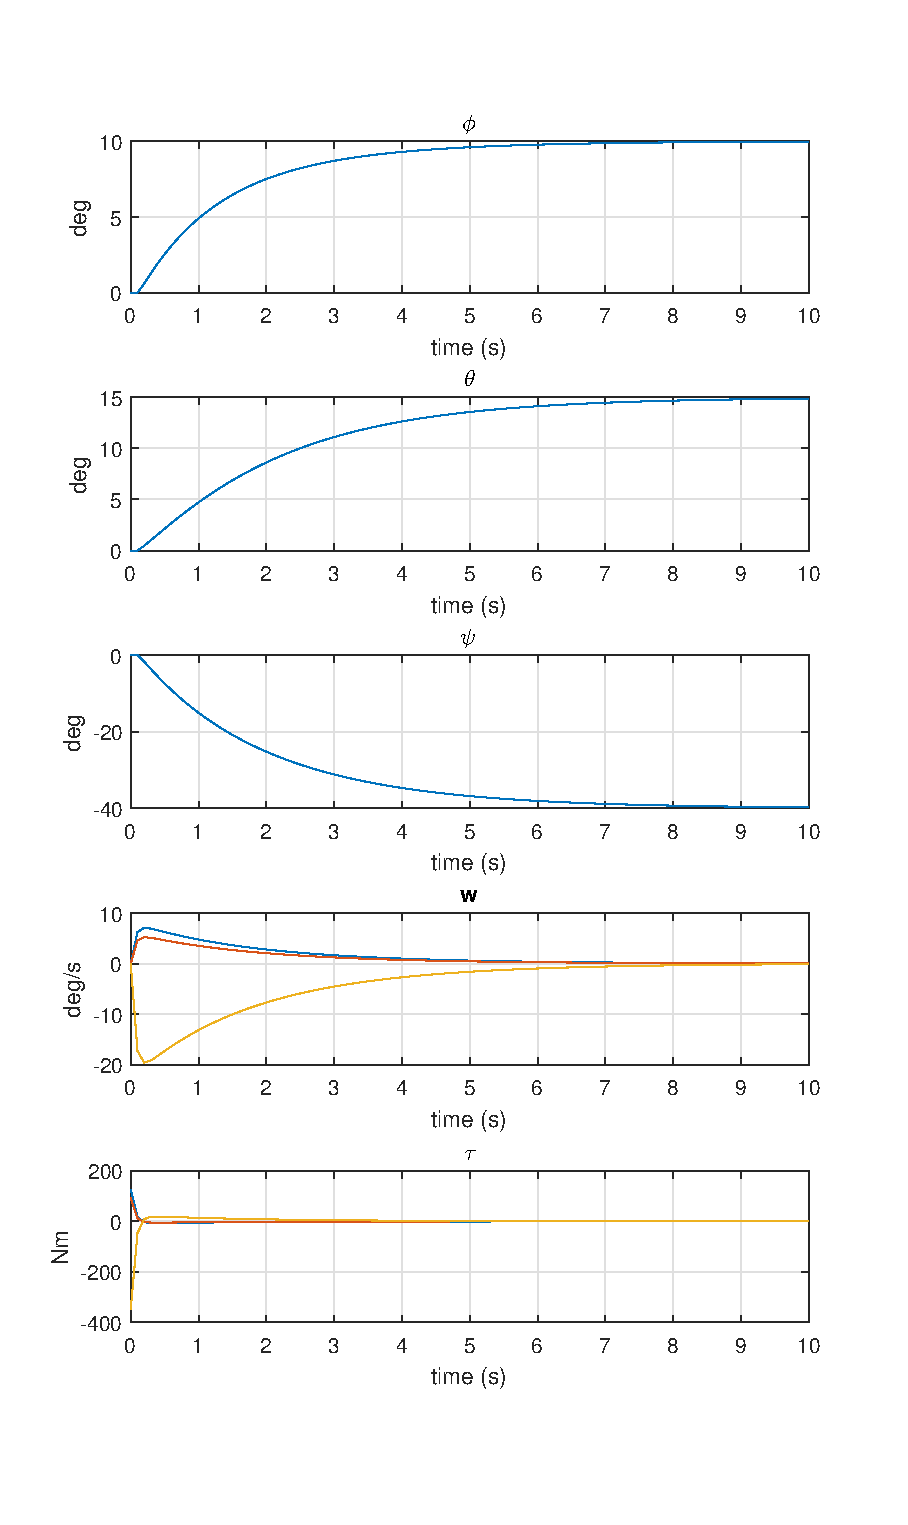
\includegraphics[width=\textwidth]{1000quat0}
		\caption{Here is a plot where the initial angles are zero and $\boldsymbol{K}_d =1000\boldsymbol{I}_{3\times 3}$ and $k_p=1000$}
		\label{fig:2a}
	\end{subfigure}
	~ %add desired spacing between images, e. g. ~, \quad, \qquad, \hfill etc. 
	%(or a blank line to force the subfigure onto a new line)
	\begin{subfigure}[b]{0.40\textwidth}
		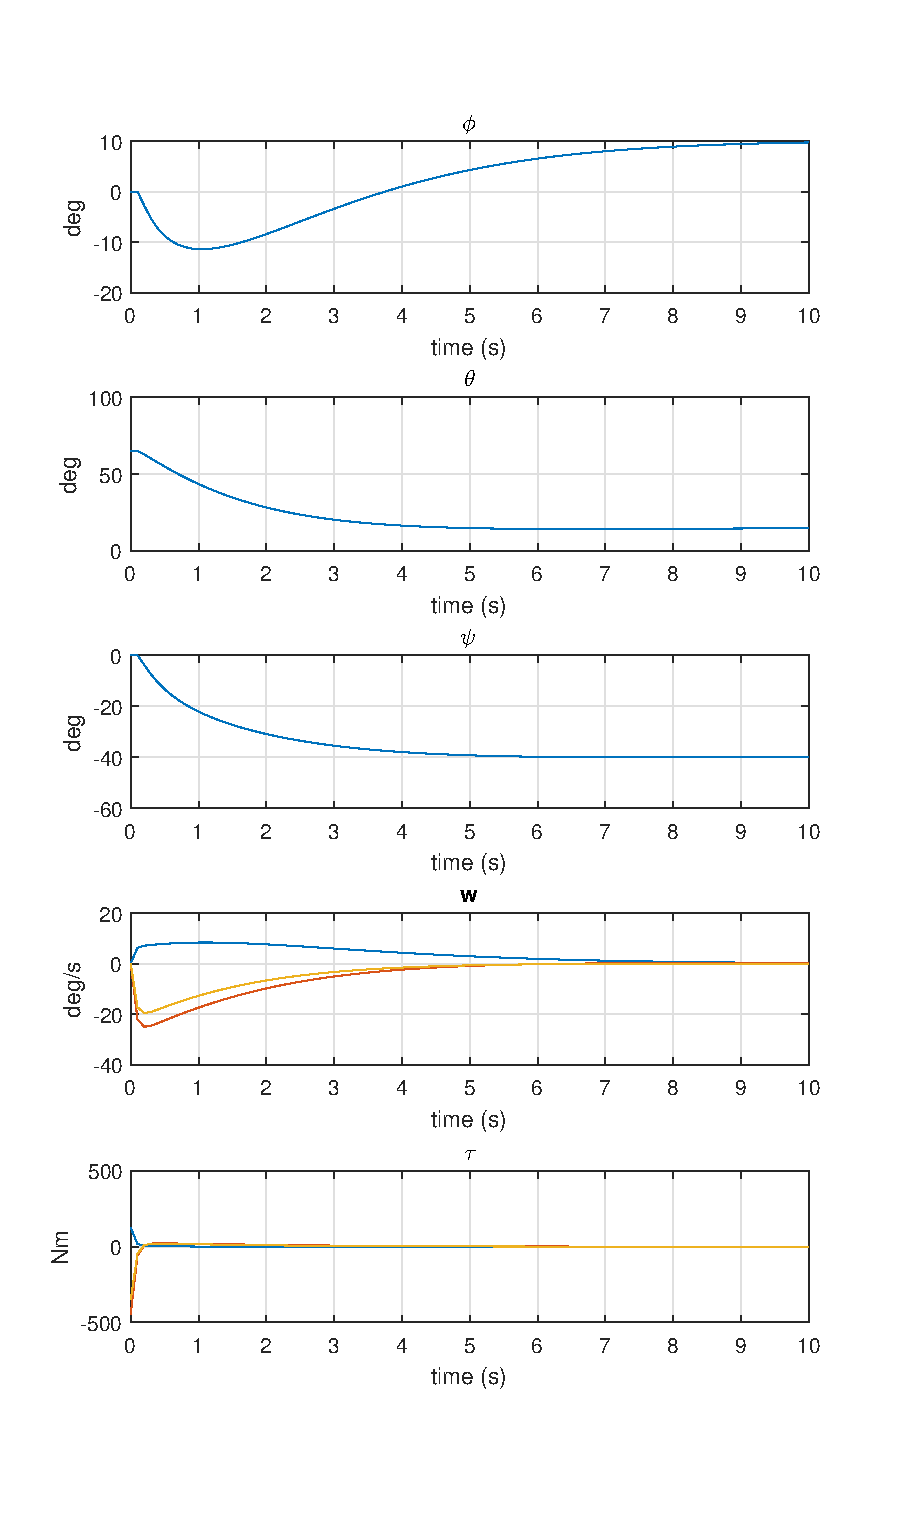
\includegraphics[width=\textwidth]{1000quat65}
		\caption{In this plot the same $\boldsymbol{K_d}$ and $k_p$ is used, but $\theta=65^\circ$ and the two other angles are zero}
		\label{fig:2b}
	\end{subfigure}
\end{figure}